\makeatletter
\def\@makechapterhead#1{%
  \vspace*{50\p@}%
  {\parindent \z@ \centering\normalfont
    \ifnum \c@secnumdepth >\m@ne
      \if@mainmatter
         \Large\bfseries \@chapapp\space \thechapter
        \par\nobreak
        \vskip 20\p@
      \fi
    \fi
    \interlinepenalty\@M
     \Large \bfseries #1\par\nobreak

    \vskip 40\p@
  }}
\def\@makeschapterhead#1{%
  \vspace*{50\p@}%
  {\parindent \z@ \centering
    \normalfont
    \interlinepenalty\@M
    \Large\bfseries  #1\par\nobreak
    \vskip 40\p@
  }}
\makeatother
\titlespacing*{\chapter}{0pt}{0pt}{12pt}

\chapter{Project Design}

\section{Requirement}

\subsection{Android SDK}

The Android software development kit (SDK) includes a comprehensive set of development tools. These include a debugger, libraries, a handset emulator based on QEMU, documentation, sample code, and tutorials. Currently supported development platforms include computers running Linux (any modern desktop Linux distribution), Mac OS X 10.5.8 or later, Windows XP or later. The officially supported integrated development environment (IDE) is Eclipse using the Android Development Tools (ADT) Plugin, though IntelliJ IDEA IDE (all editions) fully supports Android development out of the box, and NetBeans IDE also supports Android development via a plugin.[9] Additionally, developers may use any text editor to edit Java and XML files, then use command line tools (Java Development Kit and Apache Ant are required) to create, build and debug Android applications as well as control attached Android devices (e.g., triggering a reboot, installing software package(s) remotely).Enhancements to Android's SDK go hand in hand with the overall Android platform development. The SDK also supports older versions of the Android platform in case developers wish to target their applications at older devices. Development tools are downloadable components, so after one has downloaded the latest version and platform, older platforms and tools can also be downloaded for compatibility testing.

Android applications are packaged in .apk format and stored under /data/app folder on the Android OS (the folder is accessible only to the root user for security reasons). APK package contains .dex files (compiled byte code files called Dalvik executables), resource files, etc.The Android 3.1 platform (also backported to Android 2.3.4) introduces Android Open Accessory support, which allows external USB hardware (an Android USB accessory) to interact with an Android-powered device in a special "accessory" mode. When an Android-powered device is in accessory mode, the connected accessory acts as the USB host (powers the bus and enumerates devices) and the Android-powered device acts as the USB device. Android USB accessories are specifically designed to attach to Android-powered devices and adhere to a simple protocol (Android accessory protocol) that allows them to detect Android-powered devices that support accessory mode.




\subsection{Software Tools}


\subsubsection{Eclipse}
Eclipse is a multi-language software development environment comprising a base workspace and an extensible plug-in system for customizing the environment. It is written mostly in Java. It can be used to develop applications in Java and, by means of various plug-ins, other programming languages including Ada, C, C++, COBOL, Fortran, Haskell, JavaScript, Perl, PHP, Python, R, Ruby (including Ruby on Rails framework), Scala, Clojure, Groovy, Scheme, and Erlang. It can also be used to develop packages for the software Mathematica. Development environments include the Eclipse Java development tools (JDT) for Java and Scala, Eclipse CDT for C/C++ and Eclipse PDT for PHP, among others.


\subsection{System Architecture}

The Eclipse Platform uses plug-ins to provide all functionality within and on top of the runtime system, in contrast to some other applications, in which functionality is hard coded. The Eclipse Platform's runtime system is based on Equinox, an implementation of the OSGi core framework specification.

This plug-in mechanism is a lightweight software componentry framework. In addition to allowing the Eclipse Platform to be extended using other programming languages such as C and Python, the plug-in framework allows the Eclipse Platform to work with typesetting languages like LaTeX,[13] networking applications such as telnet and database management systems. The plug-in architecture supports writing any desired extension to the environment, such as for configuration management. Java and CVS support is provided in the Eclipse SDK, with support for other version control systems provided by third-party plug-ins.
With the exception of a small run-time kernel, everything in Eclipse is a plug-in. This means that every plug-in developed integrates with Eclipse in exactly the same way as other plug-ins; in this respect, all features are "created equal".[citation needed] Eclipse provides plug-ins for a wide variety of features, some of which are through third parties using both free and commercial models. Examples of plug-ins include a UML plug-in for Sequence and other UML diagrams, a plug-in for DB Explorer, and many others.

The Eclipse SDK includes the Eclipse Java development tools (JDT), offering an IDE with a built-in incremental Java compiler and a full model of the Java source files. This allows for advanced refactoring techniques and code analysis. The IDE also makes use of a workspace, in this case a set of metadata over a flat filespace allowing external file modifications as long as the corresponding workspace "resource" is refreshed afterwards.

Eclipse implements widgets through a widget toolkit for Java called SWT, unlike most Java applications, which use the Java standard Abstract Window Toolkit (AWT) or Swing. Eclipse's user interface also uses an intermediate graphical user interface layer called JFace, which simplifies the construction of applications based on SWT.Language packs developing by the "Babel project" provide translations into over a dozen natural languages.

\subsubsection{SubSub}
XXXXXXXXXXXXXXXXXXXXX 

\subsection{UML }
XXXXXXX
\subsubsection{Data Flow Diagram}

\subsubsection{0 Level}

\begin{figure} [ht]
\centering
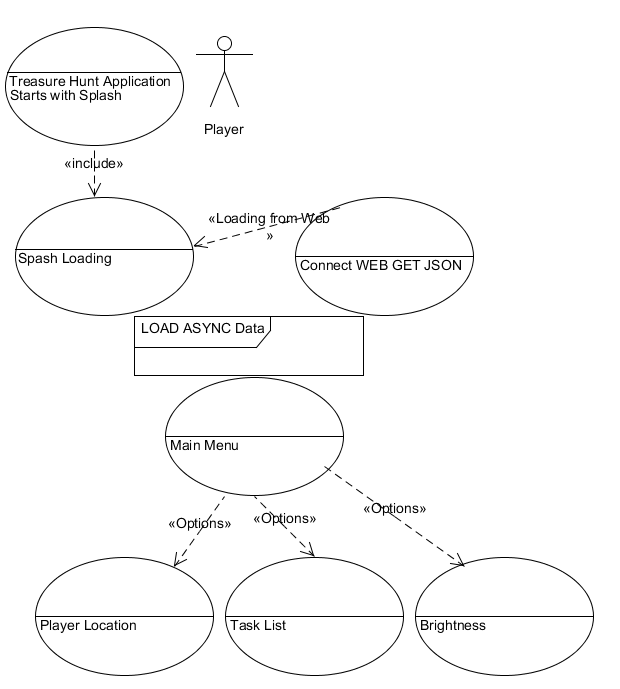
\includegraphics[scale=0.5]{dfd0}\\
\caption{DFD - 0 }
\label{the-label-for-cross-referencing}
\end{figure}



\subsection{Test Designs }